% Template GRASS newsletter - Article
% Language: Latex
%

% Head

\title{Starter Manual to Quantum GIS for GRASS GIS}
\subtitle{}
\author{GRASS Development Team}

\maketitle

\section{QUANTUM GIS INTRODUCTION}

This Manual is valid for QGIS version 0.8+ (http://www.qgis.org)
\textbf{Start QGIS}, the first time it should look like Fig.~\ref{fig:qgis000}

%\setkeys{Gin}{width=1\textwidth}
\begin{figure}[htbp]
   \centering
   %name of your graphic, without the path AND in PNG (screnshots etc)/PDF (drawings) format:
   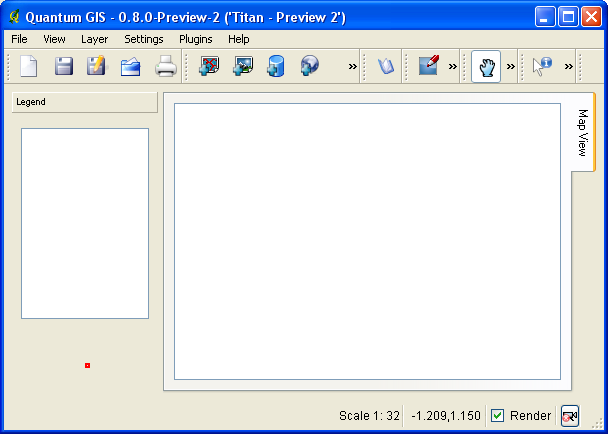
\includegraphics[scale=0.35]{qgis000.png}
   %caption of the figure
   \caption{}
   %label of the figure, which has to correspond to \ref{}:
   \label{fig:qgis000}
\end{figure}

Open some vector layers from QGIS sample data set Fig.~\ref{fig:qgis001}

%\setkeys{Gin}{width=1\textwidth}
\begin{figure}[htbp]
   \centering
   %name of your graphic, without the path AND in PNG (screnshots etc)/PDF (drawings) format:
   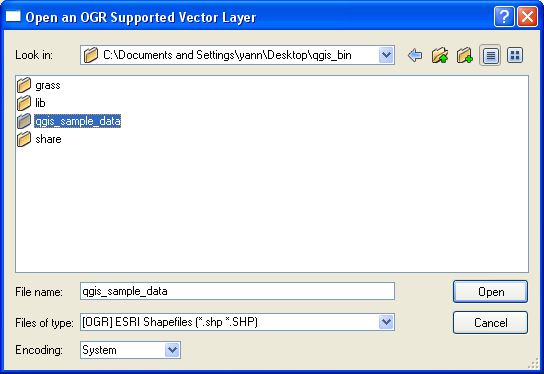
\includegraphics[scale=0.35]{qgis001.png}
   %caption of the figure
   \caption{}
   %label of the figure, which has to correspond to \ref{}:
   \label{fig:qgis001}
\end{figure}

Select all the layers (Ctrl+a) Fig.~\ref{fig:qgis002}

%\setkeys{Gin}{width=1\textwidth}
\begin{figure}[htbp]
   \centering
   %name of your graphic, without the path AND in PNG (screnshots etc)/PDF (drawings) format:
   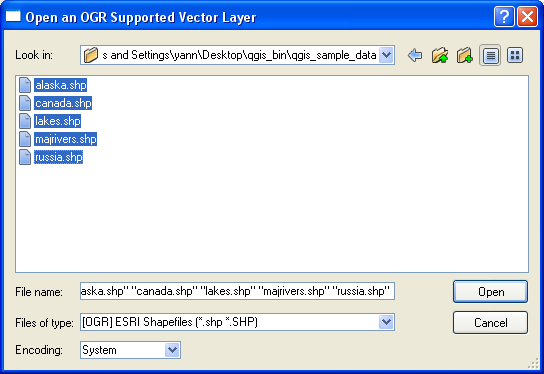
\includegraphics[scale=0.35]{qgis002.png}
   %caption of the figure
   \caption{}
   %label of the figure, which has to correspond to \ref{}:
   \label{fig:qgis002}
\end{figure}

The layers displayed should look like Fig.~\ref{fig:qgis003}

%\setkeys{Gin}{width=1\textwidth}
\begin{figure}[htbp]
   \centering
   %name of your graphic, without the path AND in PNG (screnshots etc)/PDF (drawings) format:
   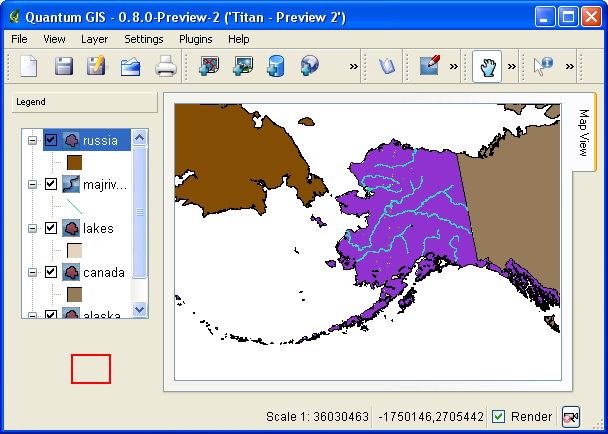
\includegraphics[scale=0.35]{qgis003.png}
   %caption of the figure
   \caption{}
   %label of the figure, which has to correspond to \ref{}:
   \label{fig:qgis003}
\end{figure}

Zoom to all layers extents... Fig.~\ref{fig:qgis004}

%\setkeys{Gin}{width=1\textwidth}
\begin{figure}[htbp]
   \centering
   %name of your graphic, without the path AND in PNG (screnshots etc)/PDF (drawings) format:
   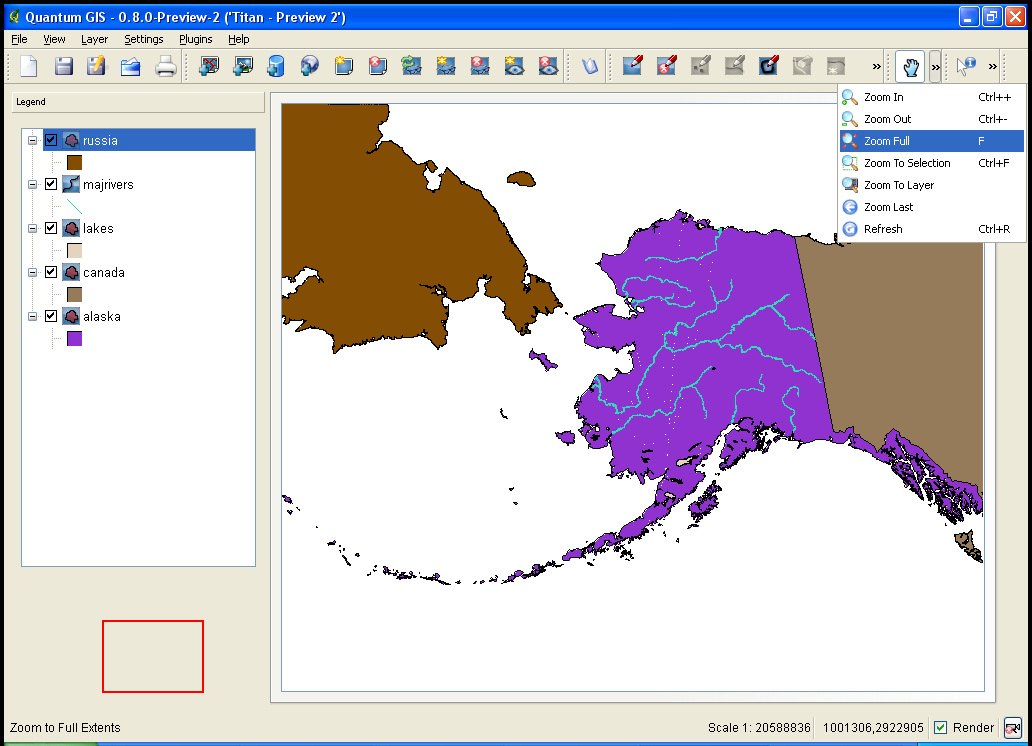
\includegraphics[scale=0.2]{qgis004.png}
   %caption of the figure
   \caption{}
   %label of the figure, which has to correspond to \ref{}:
   \label{fig:qgis004}
\end{figure}

Result after zooming to all layers Fig.~\ref{fig:qgis005}

%\setkeys{Gin}{width=1\textwidth}
\begin{figure}[htbp]
   \centering
   %name of your graphic, without the path AND in PNG (screnshots etc)/PDF (drawings) format:
   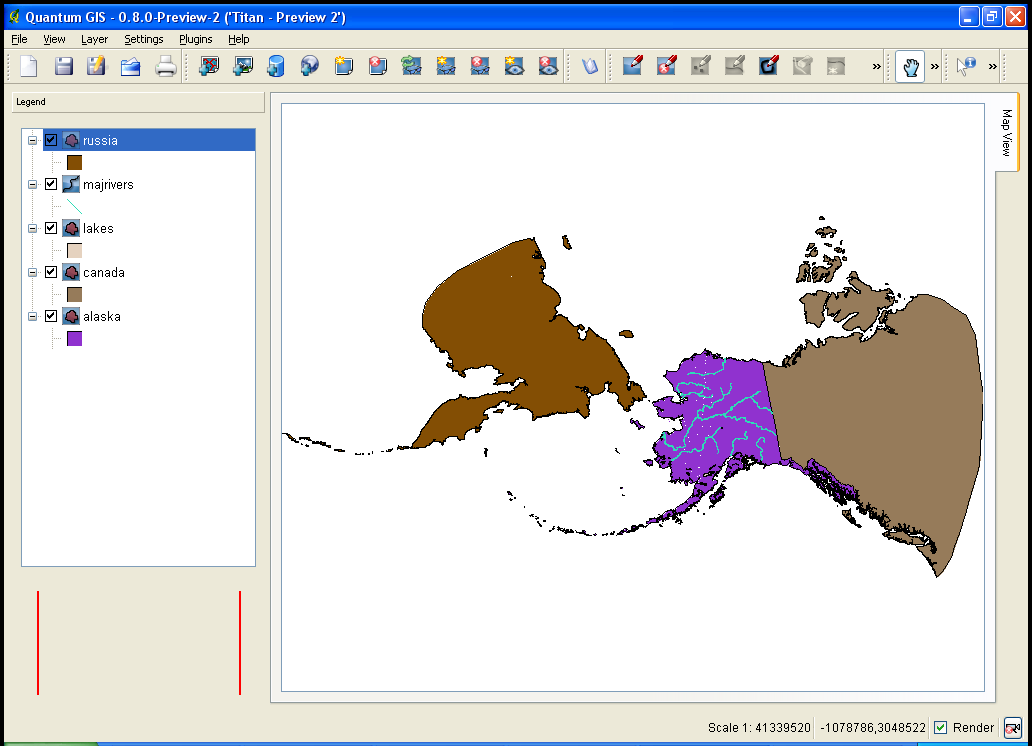
\includegraphics[scale=0.2]{qgis005.png}
   %caption of the figure
   \caption{}
   %label of the figure, which has to correspond to \ref{}:
   \label{fig:qgis005}
\end{figure}

Set the first layer in the overview frame Fig.~\ref{fig:qgis006}

%\setkeys{Gin}{width=1\textwidth}
\begin{figure}[htbp]
   \centering
   %name of your graphic, without the path AND in PNG (screnshots etc)/PDF (drawings) format:
   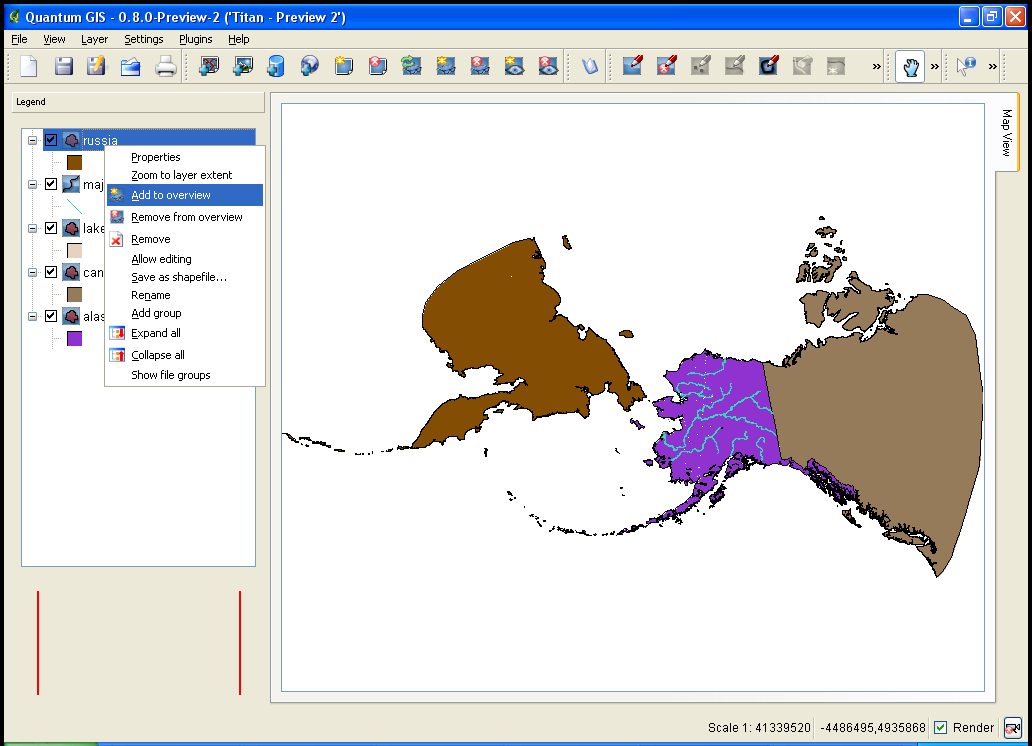
\includegraphics[scale=0.2]{qgis006.png}
   %caption of the figure
   \caption{}
   %label of the figure, which has to correspond to \ref{}:
   \label{fig:qgis006}
\end{figure}

Result... Fig.~\ref{fig:qgis007}

%\setkeys{Gin}{width=1\textwidth}
\begin{figure}[htbp]
   \centering
   %name of your graphic, without the path AND in PNG (screnshots etc)/PDF (drawings) format:
   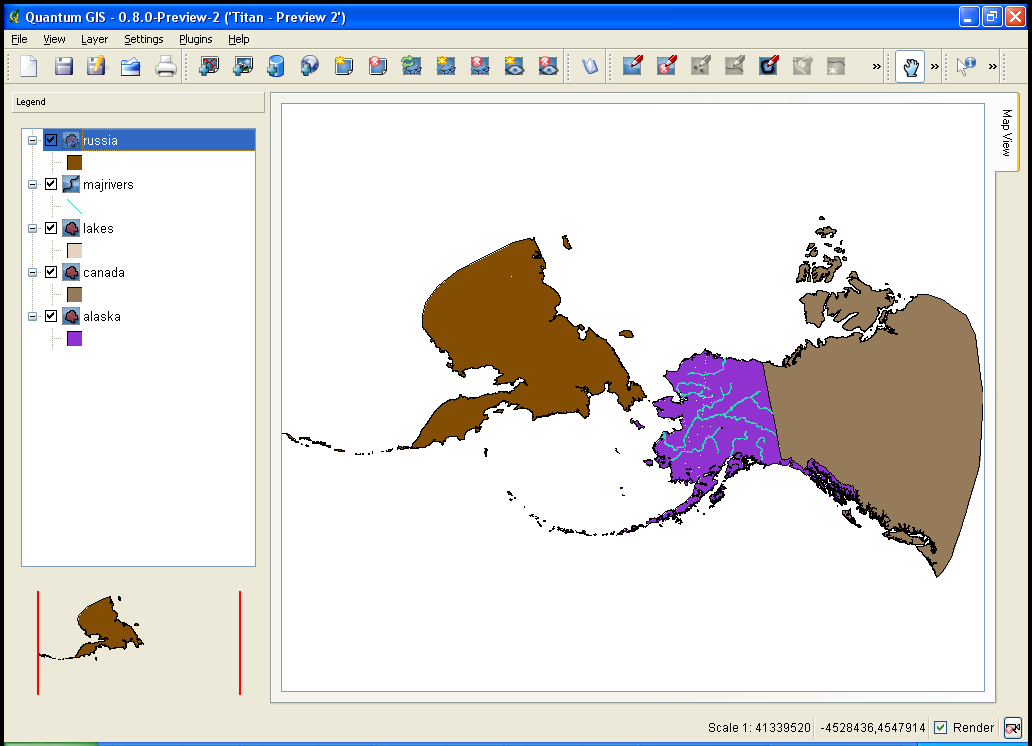
\includegraphics[scale=0.2]{qgis007.png}
   %caption of the figure
   \caption{}
   %label of the figure, which has to correspond to \ref{}:
   \label{fig:qgis007}
\end{figure}

Open the plugin menu Fig.~\ref{fig:qgis008}

%\setkeys{Gin}{width=1\textwidth}
\begin{figure}[htbp]
   \centering
   %name of your graphic, without the path AND in PNG (screnshots etc)/PDF (drawings) format:
   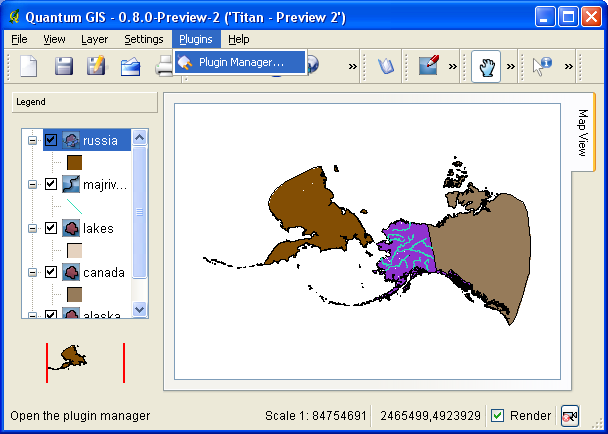
\includegraphics[scale=0.35]{qgis008.png}
   %caption of the figure
   \caption{}
   %label of the figure, which has to correspond to \ref{}:
   \label{fig:qgis008}
\end{figure}

It should look like this Fig.~\ref{fig:qgis009}

%\setkeys{Gin}{width=1\textwidth}
\begin{figure}[htbp]
   \centering
   %name of your graphic, without the path AND in PNG (screnshots etc)/PDF (drawings) format:
   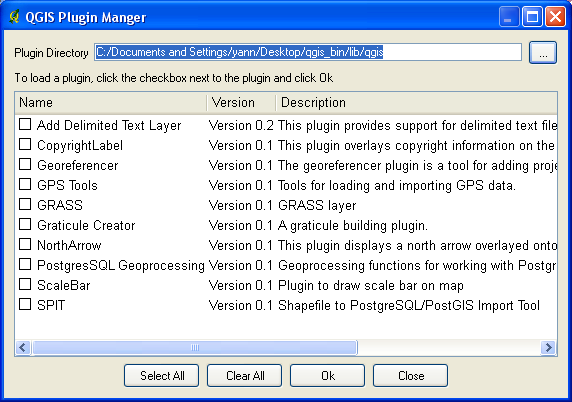
\includegraphics[scale=0.35]{qgis009.png}
   %caption of the figure
   \caption{}
   %label of the figure, which has to correspond to \ref{}:
   \label{fig:qgis009}
\end{figure}

Select those plugins Fig.~\ref{fig:qgis010}

%\setkeys{Gin}{width=1\textwidth}
\begin{figure}[htbp]
   \centering
   %name of your graphic, without the path AND in PNG (screnshots etc)/PDF (drawings) format:
   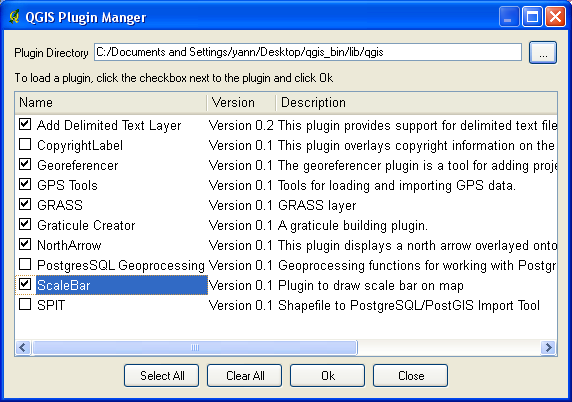
\includegraphics[scale=0.35]{qgis010.png}
   %caption of the figure
   \caption{}
   %label of the figure, which has to correspond to \ref{}:
   \label{fig:qgis010}
\end{figure}


Some new menus have appeared! Fig.~\ref{fig:qgis011}

%\setkeys{Gin}{width=1\textwidth}
\begin{figure}[htbp]
   \centering
   %name of your graphic, without the path AND in PNG (screnshots etc)/PDF (drawings) format:
   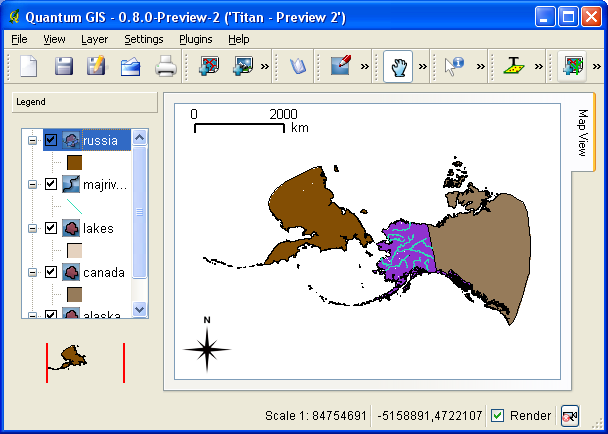
\includegraphics[scale=0.35]{qgis011.png}
   %caption of the figure
   \caption{}
   %label of the figure, which has to correspond to \ref{}:
   \label{fig:qgis011}
\end{figure}


Maximizing QGIS makes more icons appearing... Fig.~\ref{fig:qgis012}

%\setkeys{Gin}{width=1\textwidth}
\begin{figure}[htbp]
   \centering
   %name of your graphic, without the path AND in PNG (screnshots etc)/PDF (drawings) format:
   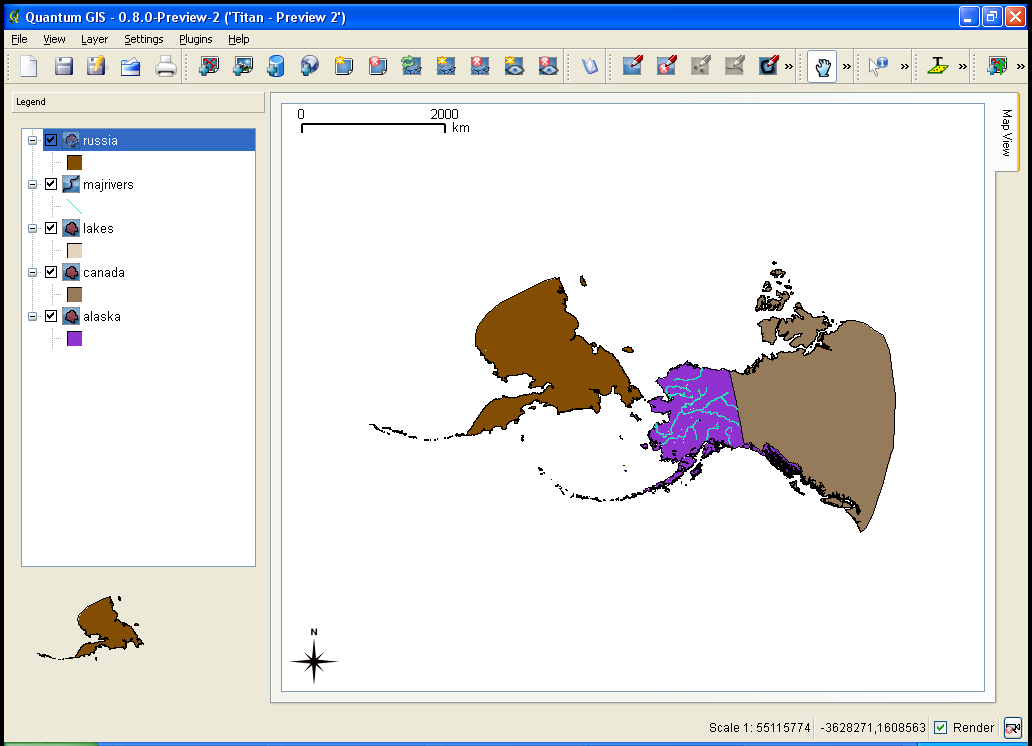
\includegraphics[scale=0.2]{qgis012.png}
   %caption of the figure
   \caption{}
   %label of the figure, which has to correspond to \ref{}:
   \label{fig:qgis012}
\end{figure}


Drag the new menus below to make them glue to a second level of
toolbars... Fig.~\ref{fig:qgis013}

%\setkeys{Gin}{width=1\textwidth}
\begin{figure}[htbp]
   \centering
   %name of your graphic, without the path AND in PNG (screnshots etc)/PDF (drawings) format:
   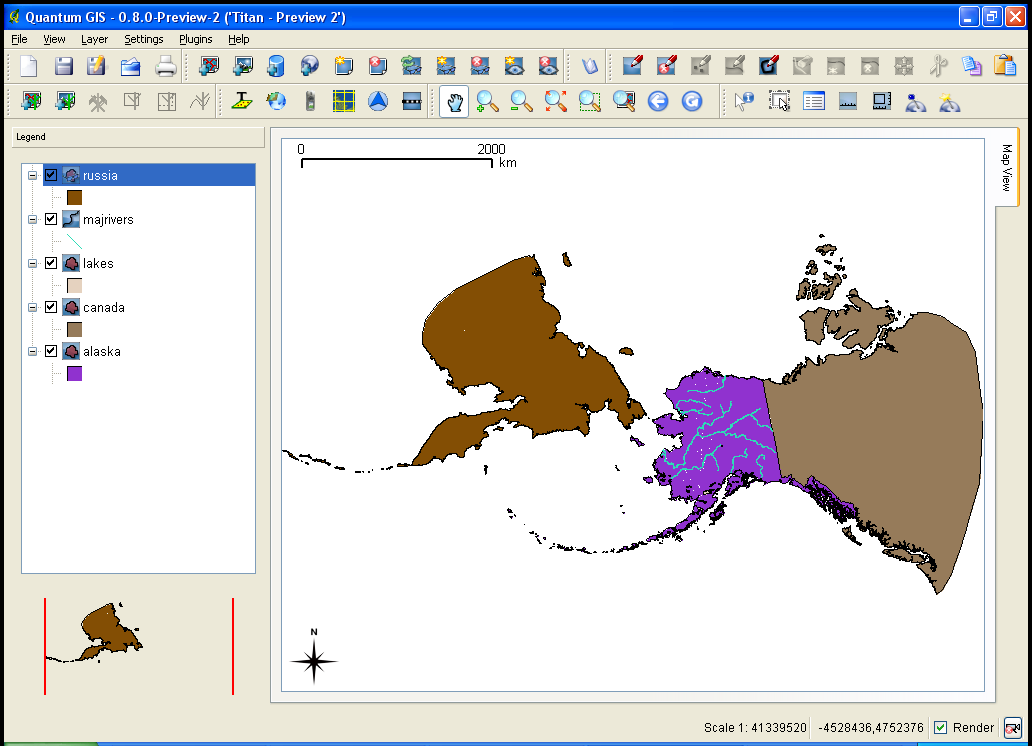
\includegraphics[scale=0.2]{qgis013.png}
   %caption of the figure
   \caption{}
   %label of the figure, which has to correspond to \ref{}:
   \label{fig:qgis013}
\end{figure}

\section{QUANTUM GIS GRASS PLUGIN}

Open a GRASS raster layer by clicking on the second button from the
left Fig.~\ref{fig:qgis014}

%\setkeys{Gin}{width=1\textwidth}
\begin{figure}[htbp]
   \centering
   %name of your graphic, without the path AND in PNG (screnshots etc)/PDF (drawings) format:
   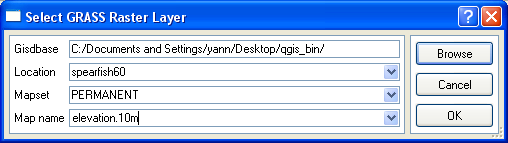
\includegraphics[scale=0.45]{qgis014.png}
   %caption of the figure
   \caption{}
   %label of the figure, which has to correspond to \ref{}:
   \label{fig:qgis014}
\end{figure}

This is the contextual menu that opens, select the Map name as
``elevation.10m'' Fig.~\ref{fig:qgis015}

%\setkeys{Gin}{width=1\textwidth}
\begin{figure}[htbp]
   \centering
   %name of your graphic, without the path AND in PNG (screnshots etc)/PDF (drawings) format:
   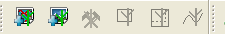
\includegraphics[scale=0.85]{qgis015.png}
   %caption of the figure
   \caption{}
   %label of the figure, which has to correspond to \ref{}:
   \label{fig:qgis015}
\end{figure}
 

This is the result of loading the GRASS Raster Layer Fig.~\ref{fig:qgis016}

%\setkeys{Gin}{width=1\textwidth}
\begin{figure}[htbp]
   \centering
   %name of your graphic, without the path AND in PNG (screnshots etc)/PDF (drawings) format:
   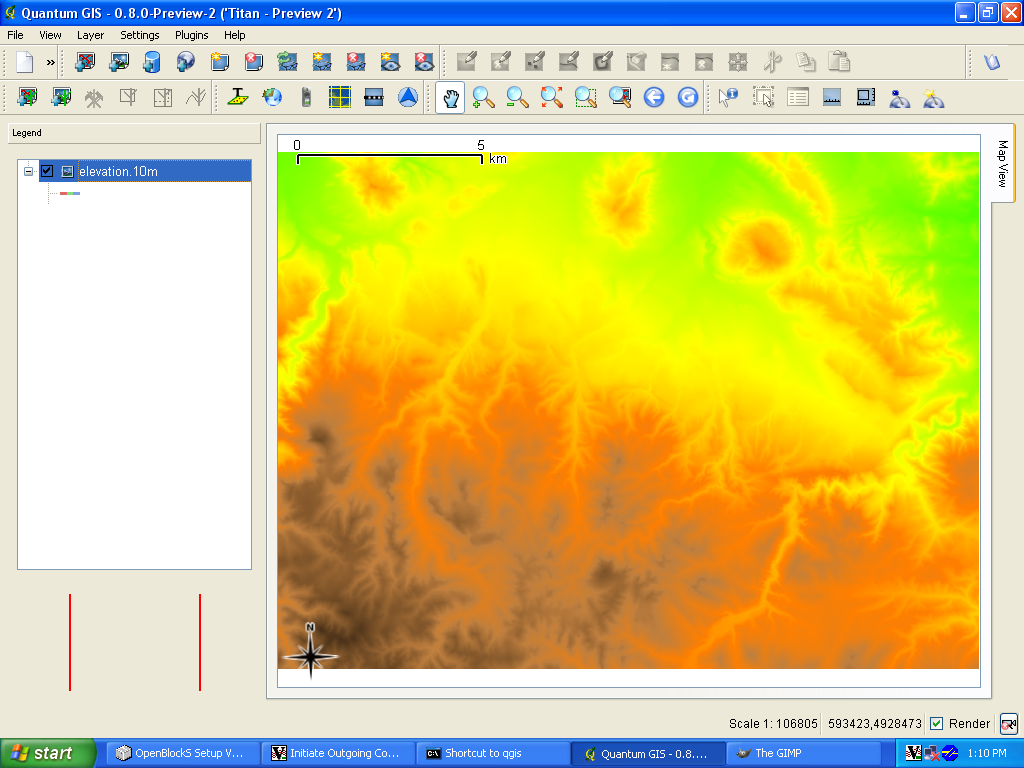
\includegraphics[scale=0.2]{qgis016.png}
   %caption of the figure
   \caption{}
   %label of the figure, which has to correspond to \ref{}:
   \label{fig:qgis016}
\end{figure}

Very similarly with other types of data, add the layer to overview Fig.~\ref{fig:qgis017}

%\setkeys{Gin}{width=1\textwidth}
\begin{figure}[htbp]
   \centering
   %name of your graphic, without the path AND in PNG (screnshots etc)/PDF (drawings) format:
   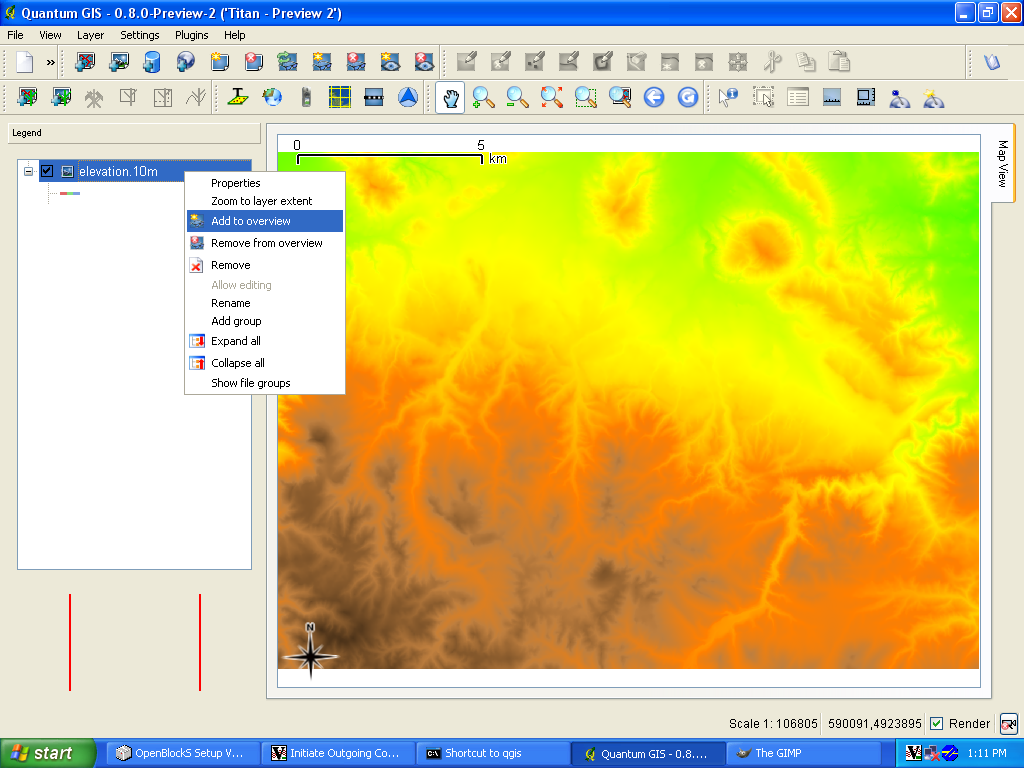
\includegraphics[scale=0.2]{qgis017.png}
   %caption of the figure
   \caption{}
   %label of the figure, which has to correspond to \ref{}:
   \label{fig:qgis0017}
\end{figure}

Result Fig.~\ref{fig:qgis018}

%\setkeys{Gin}{width=1\textwidth}
\begin{figure}[htbp]
   \centering
   %name of your graphic, without the path AND in PNG (screnshots etc)/PDF (drawings) format:
   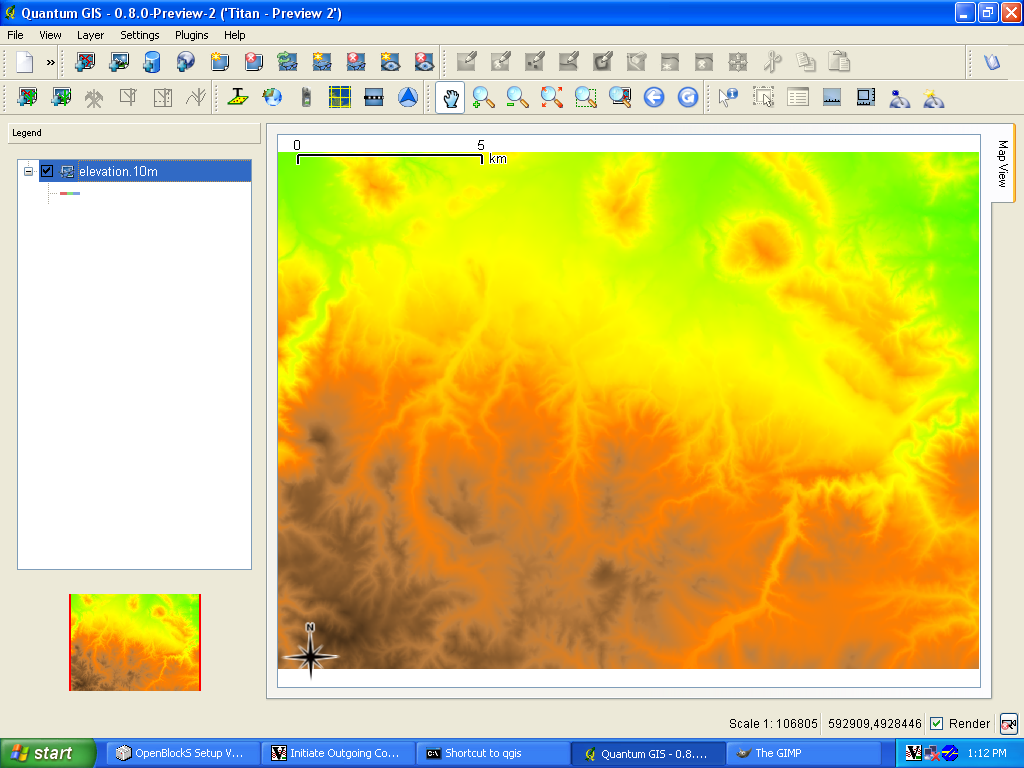
\includegraphics[scale=0.2]{qgis018.png}
   %caption of the figure
   \caption{}
   %label of the figure, which has to correspond to \ref{}:
   \label{fig:qgis018}
\end{figure}

Add a GRASS Vector Layer by selecting the first Icon from the left Fig.~\ref{fig:qgis019}

%\setkeys{Gin}{width=1\textwidth}
\begin{figure}[htbp]
   \centering
   %name of your graphic, without the path AND in PNG (screnshots etc)/PDF (drawings) format:
   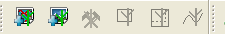
\includegraphics[scale=0.75]{qgis019.png}
   %caption of the figure
   \caption{}
   %label of the figure, which has to correspond to \ref{}:
   \label{fig:qgis019}
\end{figure}

This is the contextual menu that opens, select the Map name as
``streams'' and the layer name as ``1\_Line'' Fig.~\ref{fig:qgis020}

%\setkeys{Gin}{width=1\textwidth}
\begin{figure}[htbp]
   \centering
   %name of your graphic, without the path AND in PNG (screnshots etc)/PDF (drawings) format:
   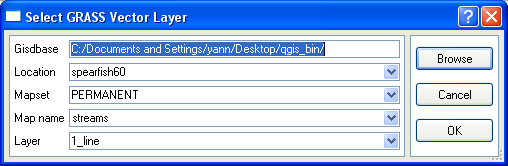
\includegraphics[scale=0.45]{qgis020.png}
   %caption of the figure
   \caption{}
   %label of the figure, which has to correspond to \ref{}:
   \label{fig:qgis020}
\end{figure}

This is the streams vector layer, open the properties by a right{}-click
on the name Fig.~\ref{fig:qgis021}

%\setkeys{Gin}{width=1\textwidth}
\begin{figure}[htbp]
   \centering
   %name of your graphic, without the path AND in PNG (screnshots etc)/PDF (drawings) format:
   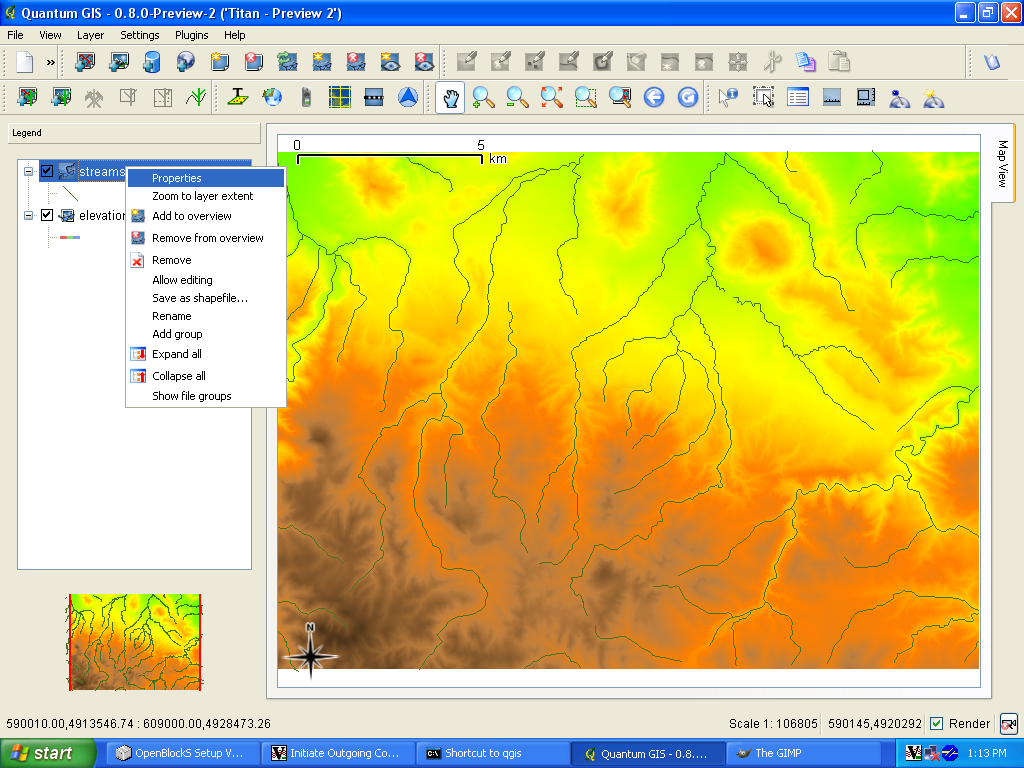
\includegraphics[scale=0.2]{qgis021.png}
   %caption of the figure
   \caption{}
   %label of the figure, which has to correspond to \ref{}:
   \label{fig:qgis021}
\end{figure}

The Properties box looks like this, and select the ``fill color'' button
to open a color selection dialog box. Change the color to a common Blue
and apply Fig.~\ref{fig:qgis022} Fig.~\ref{fig:qgis023}

%\setkeys{Gin}{width=1\textwidth}
\begin{figure}[htbp]
   \centering
   %name of your graphic, without the path AND in PNG (screnshots etc)/PDF (drawings) format:
   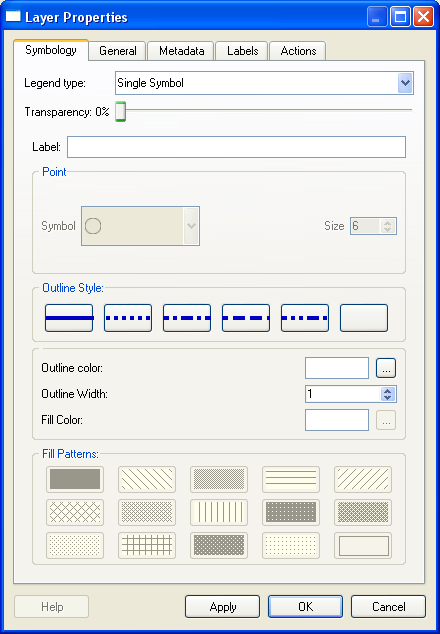
\includegraphics[scale=0.35]{qgis022.png}
   %caption of the figure
   \caption{}
   %label of the figure, which has to correspond to \ref{}:
   \label{fig:qgis022}
\end{figure}

%\setkeys{Gin}{width=1\textwidth}
\begin{figure}[htbp]
   \centering
   %name of your graphic, without the path AND in PNG (screnshots etc)/PDF (drawings) format:
   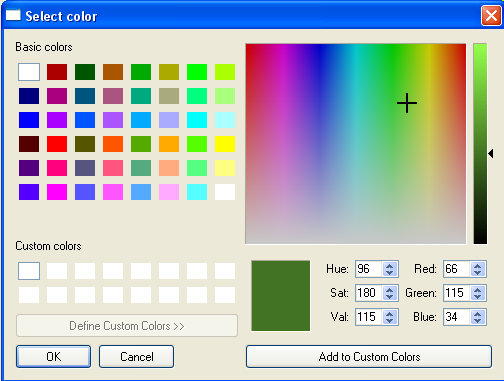
\includegraphics[scale=0.35]{qgis023.png}
   %caption of the figure
   \caption{}
   %label of the figure, which has to correspond to \ref{}:
   \label{fig:qgis023}
\end{figure}

Select the first button on the right side to start GRASS vector editing
module Fig.~\ref{fig:qgis024}

%\setkeys{Gin}{width=1\textwidth}
\begin{figure}[htbp]
   \centering
   %name of your graphic, without the path AND in PNG (screnshots etc)/PDF (drawings) format:
   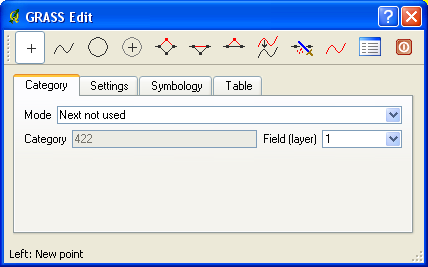
\includegraphics[scale=0.4]{qgis024.png}
   %caption of the figure
   \caption{}
   %label of the figure, which has to correspond to \ref{}:
   \label{fig:qgis024}
\end{figure}

The Edit GRASS Vector dialog box can only be opened when a vector is
selected in the main QGIS window Fig.~\ref{fig:qgis025}

%\setkeys{Gin}{width=1\textwidth}
\begin{figure}[htbp]
   \centering
   %name of your graphic, without the path AND in PNG (screnshots etc)/PDF (drawings) format:
   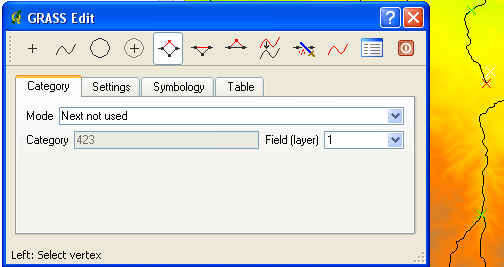
\includegraphics[scale=0.35]{qgis025.png}
   %caption of the figure
   \caption{}
   %label of the figure, which has to correspond to \ref{}:
   \label{fig:qgis025}
\end{figure}

Select the ``moving vertex'' button (5th from the
left) and move the red cross on the map Fig.~\ref{fig:qgis026}

%\setkeys{Gin}{width=1\textwidth}
\begin{figure}[htbp]
   \centering
   %name of your graphic, without the path AND in PNG (screnshots etc)/PDF (drawings) format:
   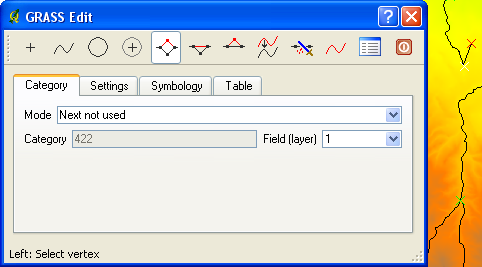
\includegraphics[scale=0.35]{qgis026.png}
   %caption of the figure
   \caption{}
   %label of the figure, which has to correspond to \ref{}:
   \label{fig:qgis026}
\end{figure}

The result should look like this (Fig.~\ref{fig:qgis026}). The last button in the toolbar will
commit the modifications to the vector layer and rebuild it Fig.~\ref{fig:qgis027}

%\setkeys{Gin}{width=1\textwidth}
\begin{figure}[htbp]
   \centering
   %name of your graphic, without the path AND in PNG (screnshots etc)/PDF (drawings) format:
   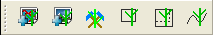
\includegraphics[scale=0.75]{qgis027.png}
   %caption of the figure
   \caption{}
   %label of the figure, which has to correspond to \ref{}:
   \label{fig:qgis027}
\end{figure}

In the launching terminal, the commit changes are described Fig.~\ref{fig:qgis028}

%\setkeys{Gin}{width=1\textwidth}
\begin{figure}[htbp]
   \centering
   %name of your graphic, without the path AND in PNG (screnshots etc)/PDF (drawings) format:
   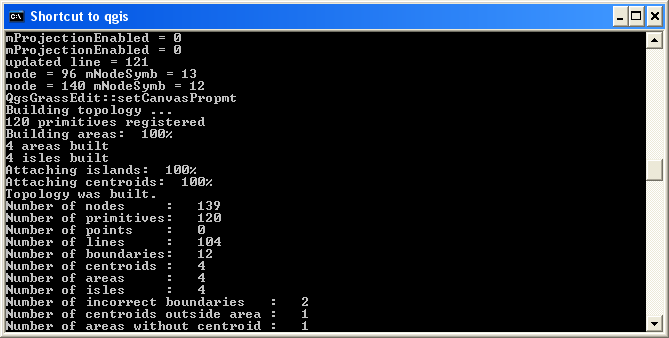
\includegraphics[scale=0.35]{qgis028.png}
   %caption of the figure
   \caption{}
   %label of the figure, which has to correspond to \ref{}:
   \label{fig:qgis028}
\end{figure}

Set GRASS plugin environment for processing... Fig.~\ref{fig:qgis029}

%\setkeys{Gin}{width=1\textwidth}
\begin{figure}[htbp]
   \centering
   %name of your graphic, without the path AND in PNG (screnshots etc)/PDF (drawings) format:
   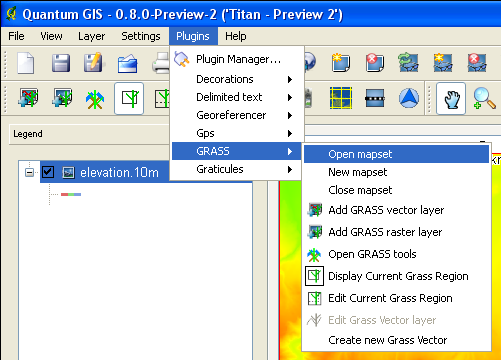
\includegraphics[scale=0.35]{qgis029.png}
   %caption of the figure
   \caption{}
   %label of the figure, which has to correspond to \ref{}:
   \label{fig:qgis029}
\end{figure}

Following this, select the 3rd icon from the left on
the GRASS toolbar. This will open the GRASS processing tool as shown
(mostly) in the next three pages. This GRASS tool is a thin
representation of the GRASS GIS capacities, but it will serve the
purpose of this introduction. It comes with a browser of the GRASS
mapset used. It also acts as a data management interface. Fig.~\ref{fig:qgis030}

%\setkeys{Gin}{width=1\textwidth}
\begin{figure}[htbp]
   \centering
   %name of your graphic, without the path AND in PNG (screnshots etc)/PDF (drawings) format:
   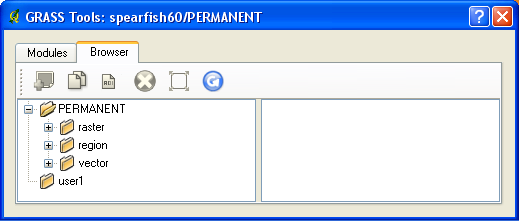
\includegraphics[scale=0.4]{qgis030.png}
   %caption of the figure
   \caption{}
   %label of the figure, which has to correspond to \ref{}:
   \label{fig:qgis030}
\end{figure}

The browser has the capacity to expand header information and metadata
pertaining to the layer selected Fig.~\ref{fig:qgis031}

%\setkeys{Gin}{width=1\textwidth}
\begin{figure}[htbp]
   \centering
   %name of your graphic, without the path AND in PNG (screnshots etc)/PDF (drawings) format:
   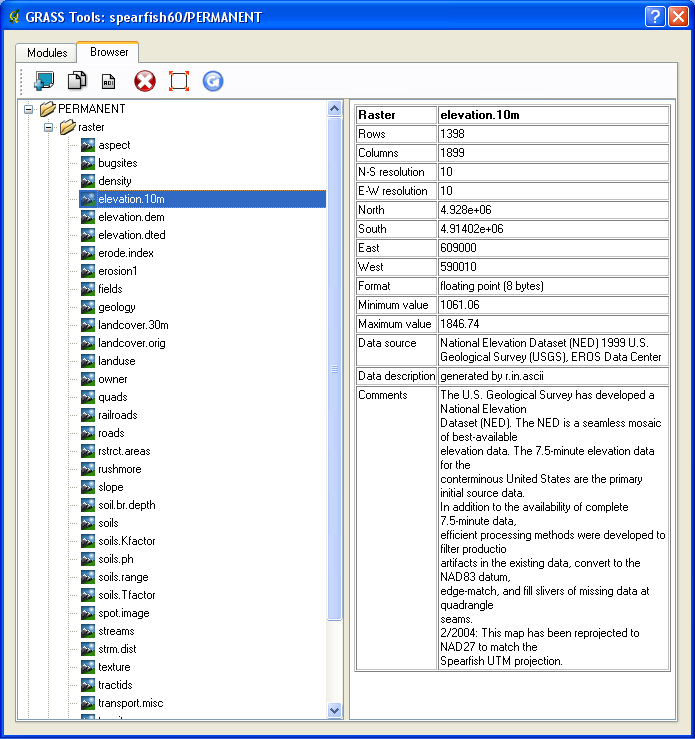
\includegraphics[scale=0.3]{qgis031.png}
   %caption of the figure
   \caption{}
   %label of the figure, which has to correspond to \ref{}:
   \label{fig:qgis031}
\end{figure}

The GRASS modules available are listed in the next two pages. More are
being ported everyday, The actual number of GRASS GIS modules exceeds
400, you can see that there is still some work to do, and the community
of volunteers are working on it Fig.~\ref{fig:qgis032} Fig.~\ref{fig:qgis033}

%\setkeys{Gin}{width=1\textwidth}
\begin{figure}[htbp]
   \centering
   %name of your graphic, without the path AND in PNG (screnshots etc)/PDF (drawings) format:
   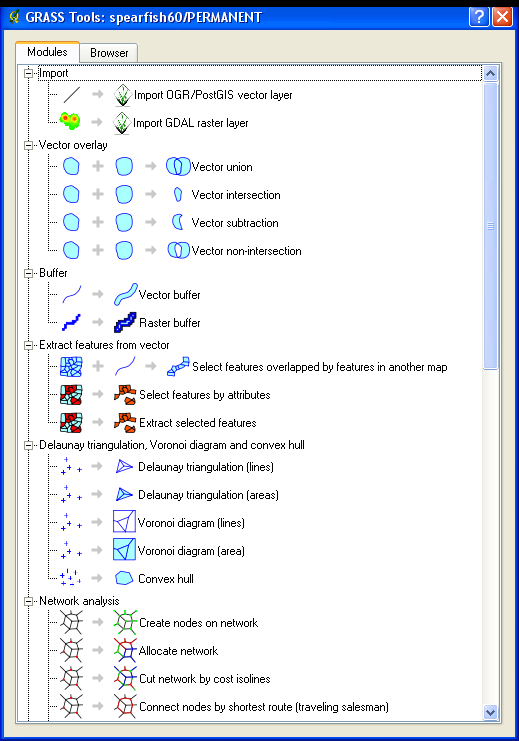
\includegraphics[scale=0.4]{qgis032.png}
   %caption of the figure
   \caption{}
   %label of the figure, which has to correspond to \ref{}:
   \label{fig:qgis032}
\end{figure}

%\setkeys{Gin}{width=1\textwidth}
\begin{figure}[htbp]
   \centering
   %name of your graphic, without the path AND in PNG (screnshots etc)/PDF (drawings) format:
   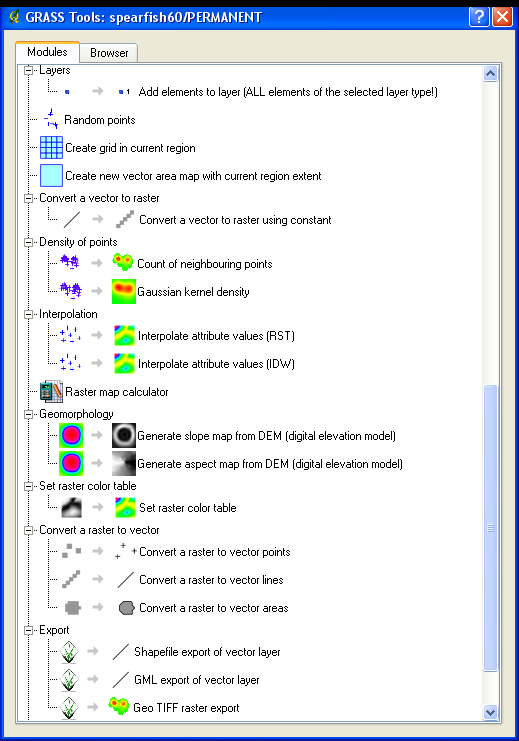
\includegraphics[scale=0.4]{qgis033.png}
   %caption of the figure
   \caption{}
   %label of the figure, which has to correspond to \ref{}:
   \label{fig:qgis033}
\end{figure}

\subsection{GRASS PLUGIN PROCESSING}

Let us create some buffers... Select buffering of vectors from the
Modules list. It should looks like this. Choose 500 meters buffer
size Fig.~\ref{fig:qgis034}

%\setkeys{Gin}{width=1\textwidth}
\begin{figure}[htbp]
   \centering
   %name of your graphic, without the path AND in PNG (screnshots etc)/PDF (drawings) format:
   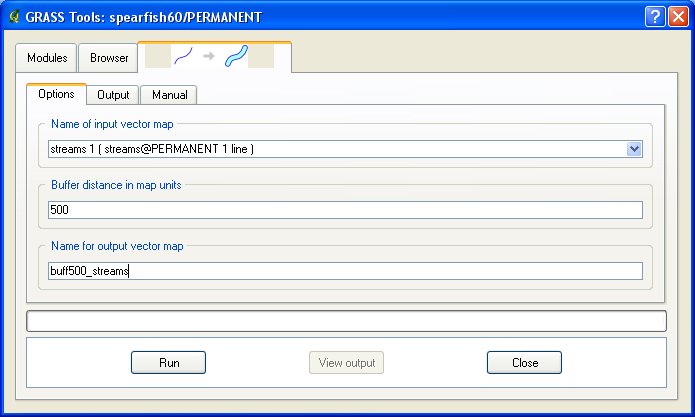
\includegraphics[scale=0.3]{qgis034.png}
   %caption of the figure
   \caption{}
   %label of the figure, which has to correspond to \ref{}:
   \label{fig:qgis034}
\end{figure}

Processing is going on... Fig.~\ref{fig:qgis035}

%\setkeys{Gin}{width=1\textwidth}
\begin{figure}[htbp]
   \centering
   %name of your graphic, without the path AND in PNG (screnshots etc)/PDF (drawings) format:
   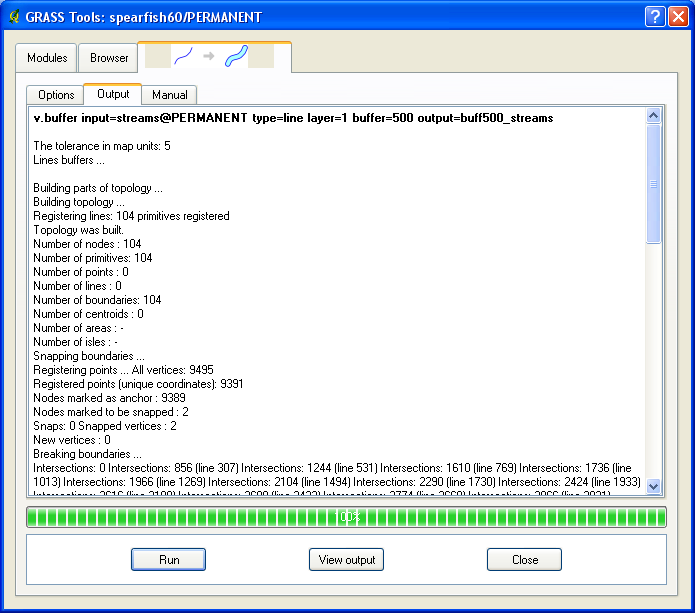
\includegraphics[scale=0.3]{qgis035.png}
   %caption of the figure
   \caption{}
   %label of the figure, which has to correspond to \ref{}:
   \label{fig:qgis035}
\end{figure}

Finishing the processing Fig.~\ref{fig:qgis036}

%\setkeys{Gin}{width=1\textwidth}
\begin{figure}[htbp]
   \centering
   %name of your graphic, without the path AND in PNG (screnshots etc)/PDF (drawings) format:
   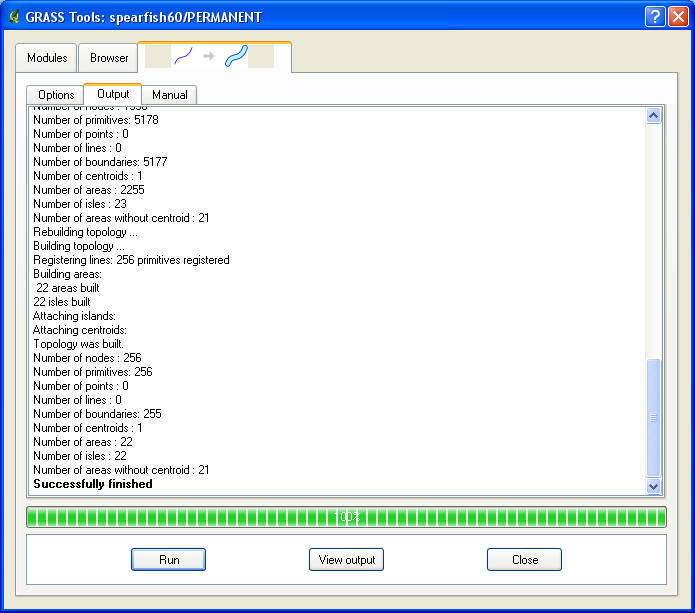
\includegraphics[scale=0.3]{qgis036.png}
   %caption of the figure
   \caption{}
   %label of the figure, which has to correspond to \ref{}:
   \label{fig:qgis036}
\end{figure}

Result should look like this (you have to load the map yourself!) Fig.~\ref{fig:qgis037}

%\setkeys{Gin}{width=1\textwidth}
\begin{figure}[htbp]
   \centering
   %name of your graphic, without the path AND in PNG (screnshots etc)/PDF (drawings) format:
   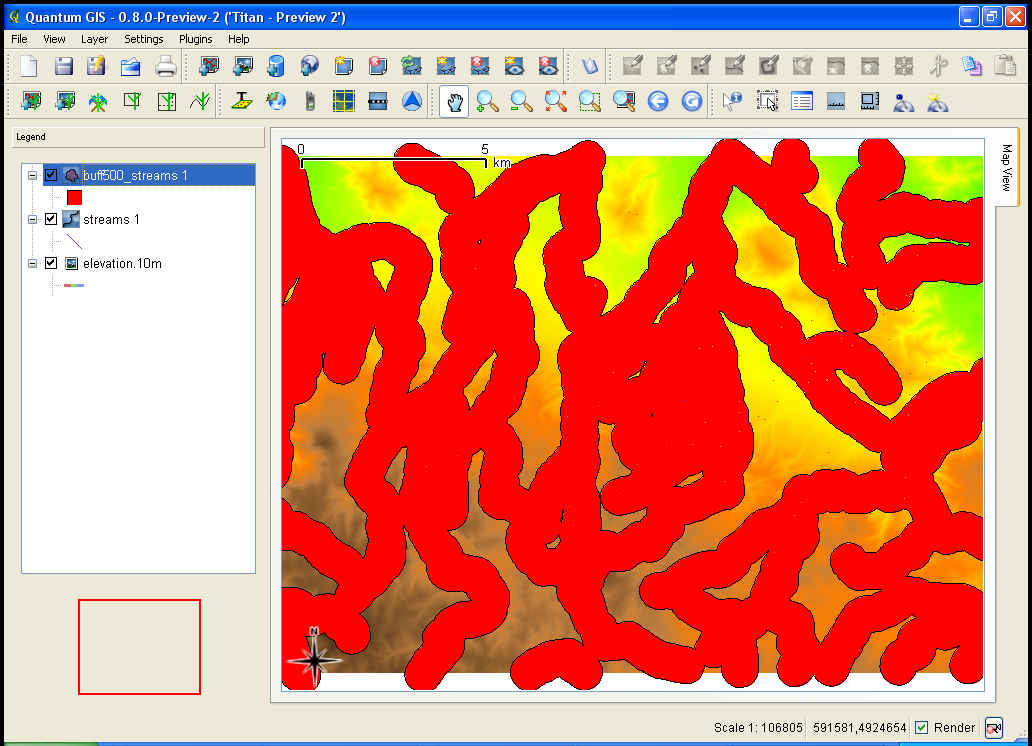
\includegraphics[scale=0.2]{qgis037.png}
   %caption of the figure
   \caption{}
   %label of the figure, which has to correspond to \ref{}:
   \label{fig:qgis037}
\end{figure}

Now create another buffer from streams but this time at 100 meters...
Like this Fig.~\ref{fig:qgis038}

%\setkeys{Gin}{width=1\textwidth}
\begin{figure}[htbp]
   \centering
   %name of your graphic, without the path AND in PNG (screnshots etc)/PDF (drawings) format:
   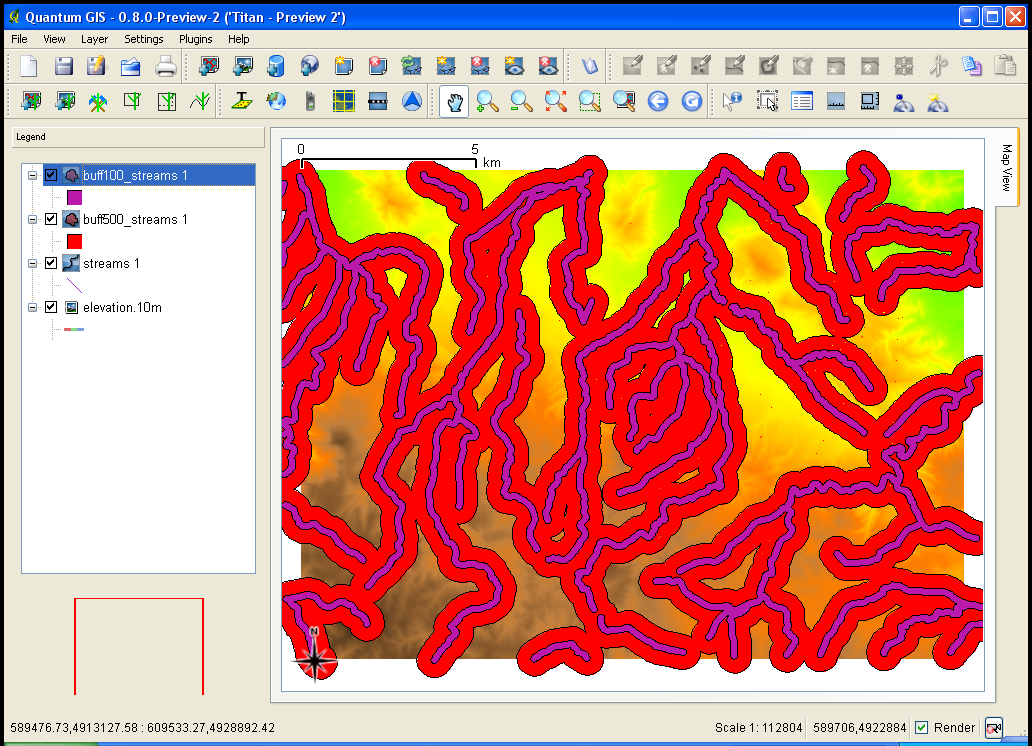
\includegraphics[scale=0.2]{qgis038.png}
   %caption of the figure
   \caption{}
   %label of the figure, which has to correspond to \ref{}:
   \label{fig:qgis038}
\end{figure}

Now we are going to subtract the 100m buffer to the 500m buffer, because
we want to exclude the streams and its proximity from our area of
selection. Find this module! Fig.~\ref{fig:qgis039}

%\setkeys{Gin}{width=1\textwidth}
\begin{figure}[htbp]
   \centering
   %name of your graphic, without the path AND in PNG (screnshots etc)/PDF (drawings) format:
   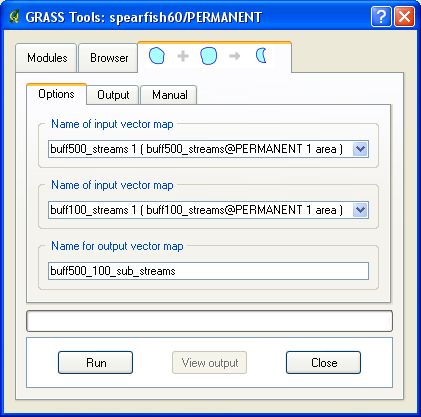
\includegraphics[scale=0.35]{qgis039.png}
   %caption of the figure
   \caption{}
   %label of the figure, which has to correspond to \ref{}:
   \label{fig:qgis039}
\end{figure}

Processing the overlay with boolean operator ``NOT'' Fig.~\ref{fig:qgis040}

%\setkeys{Gin}{width=1\textwidth}
\begin{figure}[htbp]
   \centering
   %name of your graphic, without the path AND in PNG (screnshots etc)/PDF (drawings) format:
   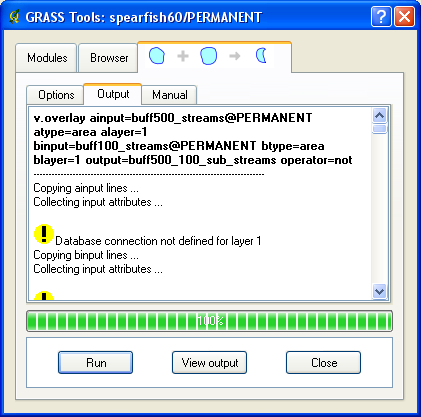
\includegraphics[scale=0.35]{qgis040.png}
   %caption of the figure
   \caption{}
   %label of the figure, which has to correspond to \ref{}:
   \label{fig:qgis040}
\end{figure}

Result is discarding all under 100m from the streams, and all above 500
meters from the streams. Fig.~\ref{fig:qgis041}

%\setkeys{Gin}{width=1\textwidth}
\begin{figure}[htbp]
   \centering
   %name of your graphic, without the path AND in PNG (screnshots etc)/PDF (drawings) format:
   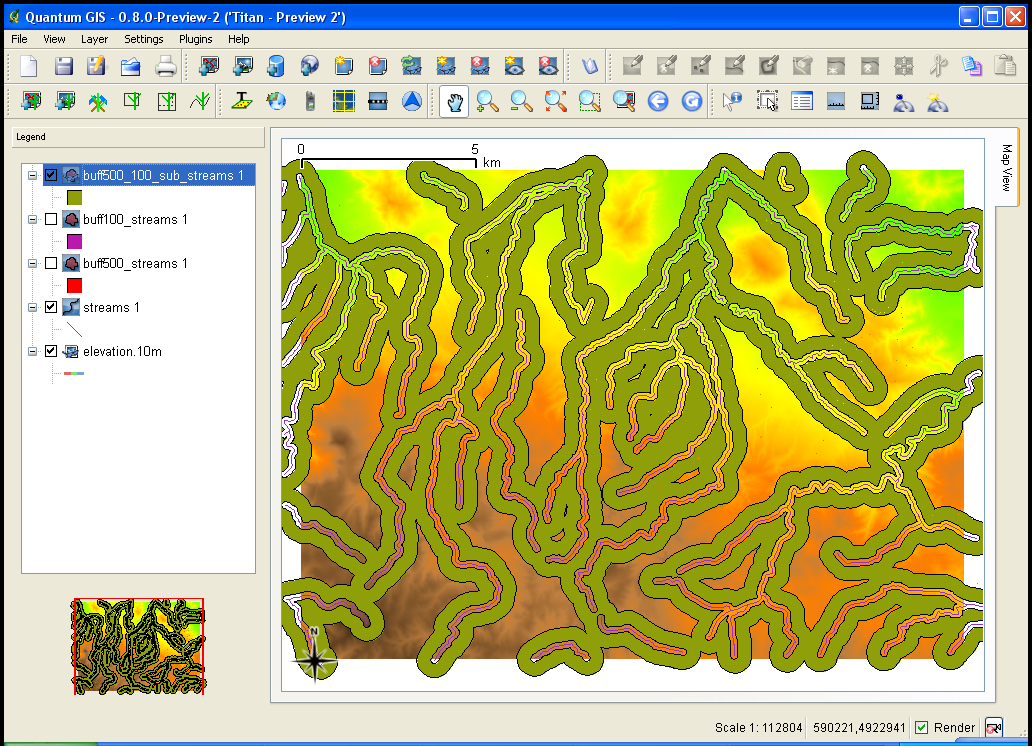
\includegraphics[scale=0.2]{qgis041.png}
   %caption of the figure
   \caption{}
   %label of the figure, which has to correspond to \ref{}:
   \label{fig:qgis041}
\end{figure}

Process an aspect map from the elevation map Fig.~\ref{fig:qgis042}

%\setkeys{Gin}{width=1\textwidth}
\begin{figure}[htbp]
   \centering
   %name of your graphic, without the path AND in PNG (screnshots etc)/PDF (drawings) format:
   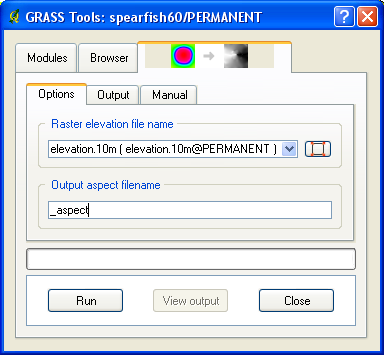
\includegraphics[scale=0.45]{qgis042.png}
   %caption of the figure
   \caption{}
   %label of the figure, which has to correspond to \ref{}:
   \label{fig:qgis042}
\end{figure}

Processing... Fig.~\ref{fig:qgis043}

%\setkeys{Gin}{width=1\textwidth}
\begin{figure}[htbp]
   \centering
   %name of your graphic, without the path AND in PNG (screnshots etc)/PDF (drawings) format:
   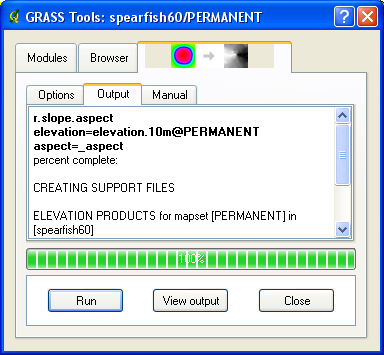
\includegraphics[scale=0.45]{qgis043.png}
   %caption of the figure
   \caption{}
   %label of the figure, which has to correspond to \ref{}:
   \label{fig:qgis043}
\end{figure}

Result Fig.~\ref{fig:qgis044}

%\setkeys{Gin}{width=1\textwidth}
\begin{figure}[htbp]
   \centering
   %name of your graphic, without the path AND in PNG (screnshots etc)/PDF (drawings) format:
   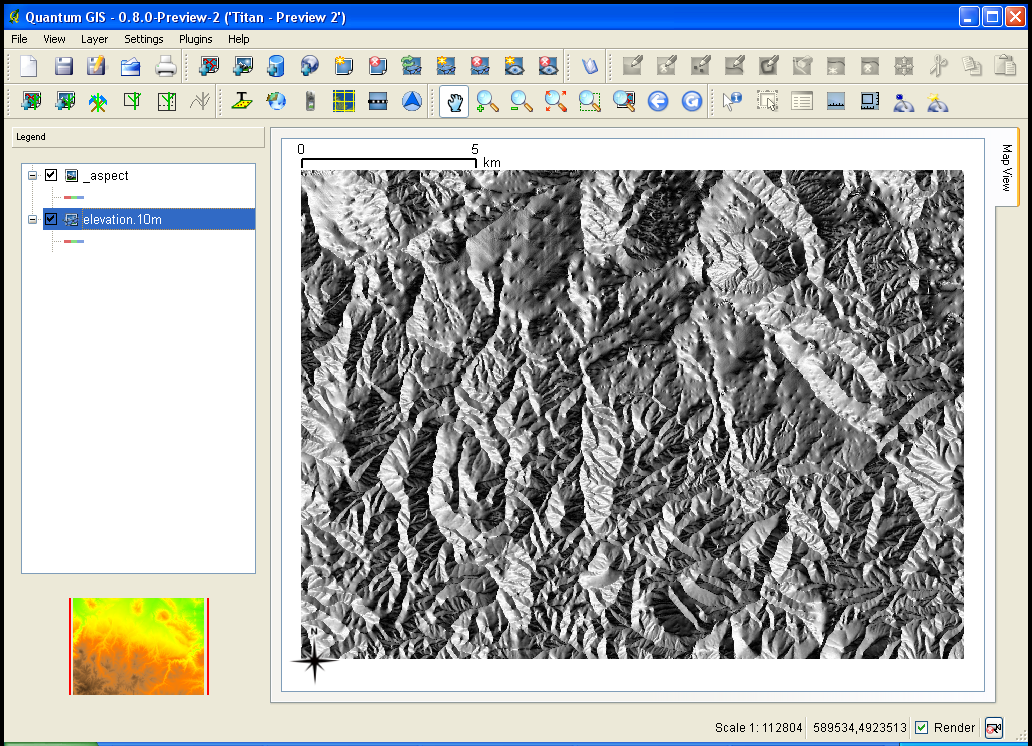
\includegraphics[scale=0.2]{qgis044.png}
   %caption of the figure
   \caption{}
   %label of the figure, which has to correspond to \ref{}:
   \label{fig:qgis044}
\end{figure}

\address{GRASS Development Team\\
  \url{http://grass.itc.it}\\
  \email{webmaster@grass.itc.it}}

%%% Local Variables: 
%%% mode: latex
%%% TeX-master: main_document.tex
%%% End:

